%!TEX root = /Users/ego/Boulot/TKZ/tkz-tab/doc/TKZdoc-tab-main.tex    
% $Id$  
% v1.0c TKZdoc-tab-adapt
%
%  Created by Alain Matthes on 2010-02-23.
%  Copyright (c) 2010 __Collège Sévigné__. All rights reserved.
\section{Personnalisation des tableaux}\label{pers}

\subsection{\texttt{\textcolor{red}{help}} :  option commune aux principales macros}

\subsubsection{\texttt{\textcolor{red}{help}} :  option de \addbs{tkzTabInit}}
Cette option permet de connaître la structure d'un tableau. \tkzname{deltacl=1} permet d'espacer un peu les points et les labels

\begin{tkzexample}[small]
	\begin{tikzpicture}
	 \tkzTabInit[deltacl=1,espcl=8,help]%
	 {$x$/1,Signe\\ de $\dfrac{1}{x}$/1.5/1.5,Variation\\ de $\ln$/2}%
	 {$0$,$+\infty$}%
	 \end{tikzpicture}
\end{tkzexample}

 
\subsubsection{\texttt{\textcolor{red}{help}} :  option de \addbs{tkzTabLine}}
Afin de mieux voir les labels il est préférable de pas employer l'option \tkzname{help} en même temps sur toutes les macros. 
\begin{tkzexample}[small]
	\begin{tikzpicture}
	 \tkzTabInit[deltacl=1,espcl=8]%
	 {$x$/1,Signe\\ de $\dfrac{1}{x}$/1.5/1.5,Variation\\ de $\ln$/2}%
	 {$0$,$+\infty$}%
	 \tkzTabLine[help]{,,}%
%  \tkzTabVar {D-/ $-\infty$,  +/$+\infty$  }
	 \end{tikzpicture}
\end{tkzexample}

\subsubsection{\texttt{\textcolor{red}{help}} :  option de \addbs{tkzTabVar}} 
Cette option montre les nodes qui sont utilisés pour le tracé des flèches de variations. Afin de ne pas multiplier les labels de nodes, seuls les nodes utilisés ont été nommés. Une flèche débute par un node  nommé \tkzname{FR} (right = droite du node) et se termine par un node nommé \tkzname{FL} (left gauche du node)
\begin{tkzexample}[small]
	\begin{tikzpicture}
	 \tkzTabInit[deltacl=1,espcl=8]%
	 {$x$/1,Signe\\ de $\dfrac{1}{x}$/1.5/1.5,Variation\\ de $\ln$/1.5}%
	 {$0$,$+\infty$}%
	 \tkzTabLine{d,+,}%
   \tkzTabVar [help]{D-/ $-\infty$,  +/$+\infty$  }
	 \end{tikzpicture}
\end{tkzexample}

Voici un exemple plus complexe

\begin{tkzexample}[small]
	\begin{tikzpicture} 
	\tkzTabInit 
	{$x$ /1, 
	$\dfrac{-1}{x^2}\ {\E}^{\left(\dfrac{1}{x}\right)}$ /1.5, 
	${\E}^{\left(\dfrac{1}{x}\right)}$ /2}% 
  {$-\infty$ ,$0$ , $+\infty$}% 
		\tkzTabLine{t,-,d,-,t} 
		\tkzTabVar[help]{ + / $1$ ,-CD+ / $0$ / $+\infty$ , - / $1$ }% 
	\end{tikzpicture}
\end{tkzexample}

ce qui donne
\begin{tkzexample}[small]
	\begin{tikzpicture} 
	\tkzTabInit 
	{$x$ /1, 
	$\dfrac{-1}{x^2}\ {\E}^{\left(\dfrac{1}{x}\right)}$ /1.5, 
	${\E}^{\left(\dfrac{1}{x}\right)}$ /2}% 
  {$-\infty$ ,$0$ , $+\infty$}% 
		\tkzTabLine{t,-,d,-,t} 
		\tkzTabVar{ + / $1$ ,-CD+ / $0$ / $+\infty$ , - / $1$ }% 
	\end{tikzpicture}
\end{tkzexample} 

La connaissance de tous ces points et nodes permet de personnaliser les tableaux. Quelques explications supplémentaires sont données dans le paragraphe suivant.

\subsection{Les structures}
\subsubsection{La structure principale}

La macro \tkzname{tkzTabInit} définit  les principaux \tkzname{nodes}. Ce sont les arguments de cette macro qui déterminent le nombre de nodes.

Par exemple, si le tableau comporte 3 lignes alors les nodes $T00$, $T01$, $T02$, $T10$, $T11$, $T12$, $T03$, $T13$ et $T23$ sont créés, ainsi que $F0$, $F1$ et $F2$.  $Tij$ représente un point de la colonne $i$ et de la ligne $j$. Pourquoi cet ordre ? je n'en sais rien

\begin{tkzexample}[vbox,small]
	\begin{tikzpicture}
	\tkzTabInit[color=false,espcl=4,lgt=3]{%
	\colorbox{red}{\textcolor{white}{$\scriptscriptstyle F0$}} / 1,%
	\colorbox{red}{\textcolor{white}{$\scriptscriptstyle F1$}} / 1,%
	\colorbox{red}{\textcolor{white}{$\scriptscriptstyle F2$}} / 1}%
	{ , }%
	\foreach \ligne in {0,...,3}{%
	   \foreach \colonne in {0,1,2}{%
	      \draw[fill=blue] (T\colonne\ligne) circle(2pt) ;}}
	\draw (T00) node[above right=4pt] {\scriptsize T00};
	\draw (T01) node[above right=4pt] {\scriptsize T01};
	\draw (T02) node[above right=4pt] {\scriptsize T02};
	\draw (T03) node[above right=4pt] {\scriptsize T03};
	\draw (T20) node[above right=4pt] {\scriptsize T20};
	\draw (T21) node[above right=4pt] {\scriptsize T21};
	\draw (T22) node[above right=4pt] {\scriptsize T22};
	\draw (T23) node[above right=4pt] {\scriptsize T23};
	\draw (T10) node[above right=4pt] {\scriptsize T10};
	\draw (T13) node[above right=4pt] {\scriptsize T13};
	\draw (T11) node[above right=3pt] {\scriptsize T11};
	\draw (T12) node[above right=3pt] {\scriptsize T12};
	\tikzset{bluesty/.style={fill=blue,<-,>=latex,shorten <=2pt}}
	\draw[bluesty] (T20) -- +(2,0) node[right,blue]{ligne $0$};
	\draw[bluesty] (T21) -- +(2,0) node[right,blue]{ligne $1$};
	\draw[bluesty] (T22) -- +(2,0) node[right,blue]{ligne $2$};
	\draw[bluesty] (T23) -- +(2,0) node[right,blue]{ligne $3$};
	\draw[bluesty] (T03) -- +(0,-2) node[midway,above,sloped,blue]{colonne $0$};
	\draw[bluesty] (T13) -- +(0,-2) node[midway,above,sloped,blue]{colonne $1$};
	\draw[bluesty] (T23) -- +(0,-2) node[midway,above,sloped,blue]{colonne $2$};
	\end{tikzpicture}
\end{tkzexample}


Ainsi la structure principale de ce tableau possède exactement trois filets verticaux  et quatre horizontaux. Soient \tkzname{12} points principaux définis par les intersections et trois nodes  $F0$, $F1$ et $F2$.

\subsubsection{La structure interne}
J'appelle structure interne, l'ensemble des points et nodes qui vont être définis par les antécédents dans la partie droite du tableau.  Le second argument de la macro \tkzname{tkzTabInit} définit cette structure. Cet argument donne le nombre de labels (antécédents) qui vont être placés sur la première ligne et qui vont être les repères pour les lignes de signes et de variations.


\begin{tkzexample}[vbox,small]
	\begin{tikzpicture}
	\tkzTabInit[color=false,espcl=4,lgt=3]{%
	\colorbox{red} {\textcolor{white}{$\scriptscriptstyle F0$}} / 1,
	\colorbox{red} {\textcolor{white}{$\scriptscriptstyle F1$}} / 1,
	\colorbox{red} {\textcolor{white}{$\scriptscriptstyle F2$}} / 1}{%
	\colorbox{blue}{\textcolor{white}{$\scriptscriptstyle L1$}},
	\colorbox{blue}{\textcolor{white}{$\scriptscriptstyle L2$}},
	\colorbox{blue}{\textcolor{white}{$\scriptscriptstyle L3$}}}%
	\foreach \ligne in {0,...,3}{%
	  \foreach \colonne in {0,1,2}{%
	    \draw[fill=blue] (T\colonne\ligne) circle(2pt) ;}}
	\foreach \colonne in {1,2,3}{%
	  \draw[fill=red] (N\colonne 0) circle(2pt)%
	       node[above,red] {\scriptsize N{\colonne 0}};}
	\foreach \ligne in {1,2,3}{%
	  \foreach \colonne in {1,2,3}{%
	    \draw[fill=red] (N\colonne\ligne) circle(2pt)%
	       node[above,red] {\scriptsize N\colonne\ligne};}}
	\foreach \ligne in {0,1,2,3}{%
	  \foreach \colonne in {1,2}{%
	    \draw[fill=green] (M\colonne\ligne) circle(2pt)
	       node[below right,green] {\scriptsize M\colonne\ligne};}}
	\tikzset{redsty/.style={fill=red,<-,>=latex,shorten <=2pt}}
	\draw[redsty] (T20) -- +(2,0) node[right,red]{ligne $0$};
	\draw[redsty] (T21) -- +(2,0) node[right,red]{ligne $1$};
	\draw[redsty] (T22) -- +(2,0) node[right,red]{ligne $2$};
	\draw[redsty] (T23) -- +(2,0) node[right,red]{ligne $3$};
	\draw[redsty] (N13) -- +(0,-2) node[midway,above,sloped,red]{colonne $1$};
	\draw[redsty] (N23) -- +(0,-2) node[midway,above,sloped,red]{colonne $2$};
	\draw[redsty] (N33) -- +(0,-2) node[midway,above,sloped,red]{colonne $3$};
	\end{tikzpicture}
\end{tkzexample}


\subsubsection{La structure secondaire}
Les points $Zij$, $Sij$ sont définis à partir de la structure interne (voir le tableau précédent) mais seulement avec l'usage de la macro \tkzcname{tkzTabLine}. Les points $FRij$ et $FLij$ eux sont définis avec l'usage de la macro \tkzcname{tkzTabVar}

\begin{tkzexample}[small]
	\begin{tikzpicture} 
	\tkzTabInit 
	{$x$ /1, 
	$\dfrac{-1}{x^2}\ {\E}^{\left(\dfrac{1}{x}\right)}$ /1.5, 
	${\E}^{\left(\dfrac{1}{x}\right)}$ /2}% 
  {$-\infty$ ,$0$ , $+\infty$}% 
		\tkzTabLine[help]{t , - , d , - , t} 
		\tkzTabVar[help]{ + / $1$ ,-CD+ / $0$ / $+\infty$ , - / $1$ }% 
	\end{tikzpicture}
\end{tkzexample}
\subsubsection{Conclusion}
\begin{tikzpicture}

\tkzTabInit[color=false,espcl=4,lgt=3,deltacl=1]{%
\colorbox{red}{\textcolor{white} {$\scriptscriptstyle F0$}} / 1,
\colorbox{red}{\textcolor{white} {$\scriptscriptstyle F1$}} / 2,
\colorbox{red}{\textcolor{white} {$\scriptscriptstyle F2$}} / 2}{%
\colorbox{blue}{\textcolor{white}{$\scriptscriptstyle L1$}} ,
\colorbox{blue}{\textcolor{white}{$\scriptscriptstyle L2$}} ,
\colorbox{blue}{\textcolor{white}{$\scriptscriptstyle L3$}} }
\foreach \ligne in {0,...,3}{%
   \foreach \colonne in {0,1,2}{%
   \draw[fill=blue] (T\colonne\ligne) circle(2pt) ;}}
\draw (T00) node[left      = 4pt] {\scriptsize T00};
\draw (T01) node[left      = 4pt] {\scriptsize T01};
\draw (T02) node[left      = 4pt] {\scriptsize T02};
\draw (T03) node[left      = 4pt] {\scriptsize T03};
\draw (T20) node[right     = 4pt] {\scriptsize T20};
\draw (T21) node[right     = 4pt] {\scriptsize T21};
\draw (T22) node[right     = 4pt] {\scriptsize T22};
\draw (T23) node[right     = 4pt] {\scriptsize T23};
\draw (T10) node[above     = 4pt] {\scriptsize T10};
\draw (T13) node[below     = 4pt] {\scriptsize T13};
\draw (T11) node[above left= 3pt] {\scriptsize T11};
\draw (T12) node[above left= 3pt] {\scriptsize T12};
 \foreach \colonne in {1,2,3}
  {\draw[fill=red] (N\colonne 0) circle(2pt)%
       node[above right] {\scriptsize N{\colonne 0}};}
\foreach \ligne in {1,2,3}
{ \foreach \colonne in {1,2,3}
  {\draw[fill=red] (N\colonne\ligne) circle(2pt)%
       node[below right] {\scriptsize N\colonne\ligne};}}
\foreach \ligne in {0,1,2,3}
{ \foreach \colonne in {1,2}
    {\draw[fill=green] (M\colonne\ligne) circle(2pt)%
       node[below right] {\scriptsize M\colonne\ligne};}}
\foreach \colonne in {1,2}
   {\path (M\colonne 1) to (M\colonne 2)%
       node[midway](S\colonne 1) {};
    \draw[fill=yellow] (S\colonne 1) circle(2pt)%
       node[below right] {\scriptsize S\colonne 1};}
\foreach \colonne in {1,2,3}
  {\path (N\colonne 1) to (N\colonne 2)%
      node[midway](Z\colonne 1) {};
   \draw[fill=yellow] (Z\colonne 1) circle(2pt)%
     node[below right] {\scriptsize Z\colonne 1};}
\end{tikzpicture}

\bigskip
\begin{tabular}{ccllc}
\toprule
type &  notation &   repère & conditions & utilisation\\
\midrule
\tikz \draw[fill=red] (0,0) rectangle (0.3,0.3) node(X) {}; &   Fj &  ligne & $0\leq j\leq p$ & expressions,formules  \\
\midrule
\tikz \draw[fill=blue] (0,0) rectangle (0.3,0.3)node(X) {}; &   Li & colonne& $1\leq i\leq n$  & valeurs significatives pour les variations \\
\midrule
\tikz \draw[fill=blue] circle (2pt)node(X) {}; &%
      Tij &  colonne& $0\leq i\leq 2$ ;& structure principale du tableau\\
&               & ligne  &$0\leq j\leq p$ & il existe une ligne $0$ et une colonne $0$\\
\midrule
\tikz \draw[fill=green] circle (2pt)node(X) {}; & Nij &colonne &$1\leq i\leq n$  & structure interne du tableau \\
& & ligne &$0\leq j\leq p$ &  \\
\midrule
\tikz \draw[fill=green] circle (2pt)node(X) {}; &   Mij &colonne &$1\leq i\leq n$ &  structure interne du tableau \\
& & ligne &$0\leq j\leq p$ & \\
\midrule
\tikz \draw[fill=yellow] circle (2pt)node(X) {}; &   Sij &colonne &$1\leq i\leq n$ & structure secondaire du tableau  \\
& & ligne &$1\leq j\leq q$ & \\
\midrule
\tikz \draw[fill=yellow] circle (2pt)node(X) {};& Zij &colonne &$1\leq i\leq n$ & structure secondaire du tableau \\
& & ligne &$1\leq j\leq q$ & \\
\midrule
\end{tabular}


\subsection{Ajustement des dimensions}
Nous avons vu précédemment que l'on pouvait modifier certaines dimensions à l'aide de l'emploi d'options. Le code du tableau suivant utilise les structures du tableau

\begin{tkzexample}[small]
	\begin{tikzpicture}
		 \tkzTabInit
		    {$x$ /  1}
		    {$a_1$ ,  $a_2$ , $a_3$}
		\begin{scope}[arstyle/.style={>=latex,#1,<->}] 
		  \draw[arstyle=blue] (N10) to node[above,color=blue]%
			     {\scriptsize $ espcl = 2$ cm} (N20);
			\draw[arstyle=blue] (N20) to node[above,color=blue]%
				   {\scriptsize $ espcl = 2$ cm} (N30);
			\draw[arstyle=red] (T10) to node[above=12pt,color=red]%
			     {\scriptsize $ deltacl = 0,5$ cm} (N10);
			\draw[arstyle=red] (N30) to node[above=12pt,color=red]%
			     {\scriptsize $ deltacl = 0,5$ cm} (T20);
			\draw[arstyle=blue] (T00) to node[above,color=blue]%
			     {\scriptsize $ lgt = 2$ cm} (T10);
		\end{scope}
	\end{tikzpicture}
\end{tkzexample}

\subsubsection{\texttt{\textcolor{red}{scale}} permet d'ajuster la taille d'un tableau}
\index{scale}


\begin{tkzexample}[width=7cm,small]
\begin{tikzpicture}[scale=.8]
  \tkzTabInit[lgt=3]{ $x$ / 1 , $\ln(x)$ /2}
                    { $0$  , $+\infty$ }
\end{tikzpicture}
\end{tkzexample}  

Il est aussi possible d'utiliser  \tkzname{xscale} et \tkzname{yscale}.

\begin{tkzexample}[width=7cm,small]
\begin{tikzpicture}[xscale=.8,yscale=1.5]
  \tkzTabInit[lgt=3]{ $x$ / 1 , $\ln(x)$ /2}
                    { $0$  , $+\infty$ }
\end{tikzpicture}
\end{tkzexample}  


\subsection{Exemples d'utilisation}
\subsubsection{Une croix sur un tableau}

\begin{tkzexample}[vbox,small]
\begin{tikzpicture}
 \tkzTab{$x$ / 1, $f'(x)$ / 1.5, $f(x)$ / 3}%
     {$-5$ , $-2$ , $1$ , $+\infty$}%
 {d,+,0,-,0,+,}
 { D-/                / $-\infty$ ,%
    +/ $\dfrac{2}{3}$ / ,%
    -/ $0$            / ,%
    +/ $+\infty$      / }%
 \draw[line width=2pt,red] (T00) to (T23);
 \draw[line width=2pt,red] (T03) to (T20);
\end{tikzpicture}
\end{tkzexample}  

\subsubsection{Une croix sur une case}

L'intérêt est de faciliter la personnalisation d'un tableau. Par exemple, si nous souhaitons ajouter un tracé comme une croix dans une case, on peut procéder ainsi :

\begin{tkzexample}[small]
\begin{tikzpicture}
\tkzTabInit%
   {$x$                   /1,
    $x^2-3x+2$            /1,
    $(x-\E)\ln x$   /1}
   {$0$  , $\E$  , $+\infty$}
   \draw[red] (T12) -- (T23);
   \draw[red] (T13) -- (T22);
\end{tikzpicture}
\end{tkzexample}  

\subsubsection{Mise en évidence de signes}
\medskip
On peut ainsi placer des signes sur la seconde ligne qui n'a pas été mise en forme par \tkzname{tkzTabLine} mais en connaissant un peu la programmation à l'aide de \TIKZ.

    \begin{tkzexample}[code only]
      \path (M11)--(M12) node[midway,draw,fill=red!10] {-};
      \path (M31)--(M32) node[midway,draw,fill=blue!10] {+};
    \end{tkzexample}
    
  \begin{tkzexample}[small]
	  \begin{tikzpicture}
	    \tkzTabInit{$x$ / 1, $\dfrac{2x}{x^2-1}$ /1}
	               {$-\infty$ , $-1$ , $1$ , $+\infty$}
	    \path (M11)--(M12) node[midway,draw,fill=red!10] {-};
	    \path (M31)--(M32) node[midway,draw,fill=blue!10] {+};
	  \end{tikzpicture}
  \end{tkzexample}

mais on peut aussi utiliser un node de la structure secondaire pour cela on utilise 
\begin{tkzexample}[]
	\tkzname{tkzTabLine}[help] \end{tkzexample}

\begin{tikzpicture}
  \tkzTabInit{$x$ / 1, $\dfrac{2x}{x^2-1}$ /1}
             {$-\infty$ , $-1$ , $1$ , $+\infty$}
  \tkzTabLine[help]{,,,,,,}
\end{tikzpicture}

Ensuite il reste à créer des nodes
\begin{tkzexample}[code only]
	  \node[draw,fill=red!10] at (S11) {-};
	  \node[draw,fill=red!10] at (S31) {+}; \end{tkzexample}

  
  
\begin{tkzexample}[small]
\begin{tikzpicture}
  \tkzTabInit{$x$ / 1, $\dfrac{2x}{x^2-1}$ /1}
             {$-\infty$ , $-1$ , $1$ , $+\infty$}
  \tkzTabLine{,,,,,,}
  \node[draw,fill=red!10] at (S11) {-};
  \node[draw,fill=red!10] at (S31) {+};
\end{tikzpicture}
\end{tkzexample}
  
\subsubsection{Structure principale : hachurer une zone}
  
On veut par exemple hachurer une zone mais vous ne connaissez pas la notation des nodes. Il suffit de passer \tkzname{help} en option. On obtient ainsi l'emplacement et les noms des nodes.
  
\begin{tkzexample}[code only]
	\begin{tikzpicture}
	\tkzTabInit[help,deltacl=1]{$x$ / 1, $\dfrac{2x}{x^2-1}$ /1,$\ln{(x^2-1)}$/1}
	                 {$-\infty$ , $-1$ , $1$ , $+\infty$}
	\end{tikzpicture}
\end{tkzexample}


\medskip
On peut  hachurer un rectangle par 

    \begin{tkzexample}[code only]
    \pattern[pattern=north west lines] (N21) rectangle (N33);
    \end{tkzexample}
    
    
\begin{tkzexample}[small]
\begin{tikzpicture}
  \tkzTabInit{$x$ / 1 , $\ln{(x^2-1)}$/1}
             {$-\infty$ , $-1$ , $1$ , $+\infty$}
  \pattern[pattern=north west lines] (N21) rectangle (N32);
\end{tikzpicture}
\end{tkzexample}

  

\subsubsection{Mise en évidence de certaines zones}

Afin de mettre en évidence le signe d'une expression du second degré, il est possible de mettre en couleur les parties extérieures. \tkzcname{draw[fill=Red!80,opacity=0.4](N11) rectangle (N22);}. La syntaxe est celle de \TIKZ. Un rectangle est défini par deux sommets opposés. 

\begin{tkzexample}[vbox,small]
\begin{tikzpicture}
 \tkzTabInit[deltacl=1,lgt=3,espcl=2]%
   {$x$ /1,$x^2-3x+2$ /1}%
   {$-\infty$ , $1$ , $2$, $+\infty$}%
 \tkzTabLine {t,+,0,-,0,+,t}
 \draw[fill=Red!80,opacity=0.4](N11) rectangle (N22);
 \draw[fill=Red!80,opacity=0.4](N31) rectangle (N42);
\end{tikzpicture}
\end{tkzexample}  

\subsubsection{Mise en évidence de valeurs}
\begin{tkzexample}[vbox,small]
\begin{tikzpicture}
\tkzTab
{$x$                                                       /1,
$\dfrac{-1}{x^2}\ {\E}^{\left(\dfrac{1}{x}\right)}$ /1.5,
${\E}^{\left(\dfrac{1}{x}\right)}$                  /2}%
{$-\infty$ ,$0$ , $+\infty$}%
{t,-, ,-,t}
{ + /  $1$ , -CD+ / \colorbox{red}{\textcolor{white}{$0$}} / $+\infty$ , - / $1$ }%
 \node[draw,inner sep=2pt,circle,fill=yellow] at (Z21) {$0$} ;
\end{tikzpicture}
\end{tkzexample}  

\subsubsection{Mise en évidence de limites}

\begin{tkzexample}[vbox,small]
\begin{tikzpicture}
 \tkzTabInit[espcl=8]%
 {$x$/1 , Variation\\ de $\ln$/2}%
 {$0$,$+\infty$}%
 \tkzTabVar {D-/ $-\infty$, +/$+\infty$ }
 \draw[opacity=.3,fill=red] (FR11) circle (10pt);
 \draw[opacity=.3,fill=red] (FL21) circle (10pt);
 \end{tikzpicture}
\end{tkzexample}  
 
 
\subsubsection{Décoration}
Il est nécessaire de charger une librairie de \TIKZ\footnote{pgf/tikz version 2.00} qui permet des actions de décoration. \NameLib{decorations.pathreplacing}

\begin{tkzexample}[code only]
	\usetikzlibrary{decorations.pathreplacing}
	\ldots
	\draw[decoration={brace,amplitude=12pt},
	      decorate,line width=2pt,red] (T10) -- (T20);\end{tkzexample}


\begin{tkzexample}[small]
	\begin{tikzpicture}
	\tkzTabInit[lgt=3,espcl=1.5]
	    {$x$                 /1,
	     $x^2-3x+2$          /1,
	     $(x-\E)\ln x$ /1}%
	    {$0$,$1$,$2$,$\E$,$+\infty$}%
	\draw[fill=Orange,opacity=.3] (N10) rectangle (N53.west);
	\draw[decoration={brace,amplitude=12pt},
	      decorate,line width=2pt,red] (T10) -- (T20);
	\end{tikzpicture}
\end{tkzexample}


\subsubsection{Avec de la couleur}
\begin{tkzexample}[vbox,small]
\begin{tikzpicture}
    \tkzTabInit[color,colorC = blue!30,colorL = orange!50,
                colorT = green!30,colorV = red!50,espcl=8]
    {$x$/1,Signe\\ de $\dfrac{1}{x}$ /1.5,Variation\\ de $\ln$ /3}
    {$0$,$+\infty$}%
    \tkzTabLine{d,+,}%
    \tkzTabVar[color=red]{D-/$-\infty$ , +/$+\infty$}
    \tkzTabVal[draw]{1}{2}{0.3}{\textcolor{red}{$\text{1}$}}{\textcolor{blue}{$0$}}
    \tkzTabVal[draw]{1}{2}{0.6}{\textcolor{red}{$\text{\large e}$}}{\textcolor{blue}{$1$}}%
    \draw[fill=gray,opacity=0.6] (T11) rectangle (N13);
\end{tikzpicture}
\end{tkzexample}  


\subsubsection{Écrire dans un tableau}

Aucune restriction au niveau de l'écriture, l'exemple suivant :

\medskip
\begin{tikzpicture}
\tkzTabInit[lgt=5,espcl=3]%
      { $x$               /1,%
        Il est parfois possible d'obtenir les variations d'une fonction sans déterminer sa dérivée    /2,%
        $\ln (x) +x$     /1%
      }%
      { $0$ , $1$ , $+\infty$ }%
\end{tikzpicture}

\begin{tkzexample}[code only]
\begin{tikzpicture}
\tkzTabInit[lgt=3,espcl=4]%
      { $x$                    /1,%
        Il est parfois ...  /2,%
        $\ln (x) +x$           /1%
      }%
      { $0$ , $1$ , $+\infty$ }%
\end{tikzpicture}
\end{tkzexample}  

\subsubsection{Tableau de proportionnalité}

On utilise ici un compteur interne \tkzname{tkz@cnt@pred} du package. l' arrobase \tkzname{@} devient une lettre ordinaire à l'aide des macros \tkzname{makeatletter} et \tkzname{makeatother}. Ce compteur va servir à tracer des filets verticaux afin de séparer les antécédents et les images.

\begin{tkzexample}[vbox,small]
\begin{tikzpicture}
  \tkzTabInit[espcl=0.5]{ $x$/1,$f(x)$ /1}%
  {1,,2,,3,,4,,5,,6}%
  \tkzTabLine{5,,,,10,,,,15,,,,20,,,,25,,,,30}%
  \makeatletter
  \foreach \x in {1,...,5}{%
     \setcounter{tkz@cnt@pred}{\x}\addtocounter{tkz@cnt@pred}{\x}
     \draw (N\thetkz@cnt@pred 0.center) to (N\thetkz@cnt@pred 2.center);}
  \makeatother
  \begin{scope}[->,red,line width=1pt,>=latex']
	  \draw (M20) to [bend left] node[above]{$\times 3$} (7.5,0);
	  \draw (M22) to [bend right] node[below]{$\times 3$} (7.5,-2);
	  \draw (8,-0.25) to [post,bend left=60] node[midway,above,sloped] {$\times 5$}  (8,-1.75);
  \end{scope}
\end{tikzpicture}
\end{tkzexample}  
\endinput



